\titre{7}
\theme{trigo}
\auteur{Nathan Scheinmann}
\niveau{1M}
\source{sesamath-1M-trigo}
\type{serie}
\piments{2}
\pts{}
\annee{2425}

\contenu{
	\tcblower
	\begin{minipage}[t]{0.50\textwidth}{
	\vspace{0pt}
	Rafaël et Léo nagent pour atteindre une bouée $P$. Ils sont respectivement en position $R$ et $L$. On a $\overline{BL}=50~\text{m}$ et $\widehat{BPL}=72^\circ$. 

	Calculer la distance entre les deux nageurs arrondie au mètre. 
	}
	\end{minipage}
	\hfill
	\begin{minipage}[t]{0.45\textwidth}{
	\vspace{0pt}
	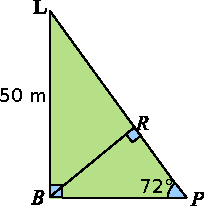
\includegraphics[scale=1]{../medias/1M/trigo/1M-exo-7}
	}
	\end{minipage}
}
\correction{

}

